


\renewcommand{\thesubsection}{\Alph{subsection}}

\section*{Appendix}

\subsection{Further Smart City definitions}

\begin{quote}[\textcite{smart1}]
“A Smart City is a city well performing built on the ‘smart’ combination of endowments and activities of self-decisive, independent and aware citizens.”
\end{quote}

\begin{quote}[\textcite{smart5}]
“Smart City is the product of Digital City combined with the Internet of Things.”
\end{quote} 

To understand this quote one definition for Digital City follows: 

\begin{quote}[\textcite{digital1}]
“A Digital City has at least two plausible meanings: (1) a city that is being transformed or re-oriented through digital technology and (2) a digital representation or reflection of some aspects of an actual or imagined city.” 
\end{quote}

\begin{quote}[\textcite{smart6}]
“Concept of a Smart City where citizens, objects, utilities, etc., connect in a seamless manner using ubiquitous technologies, so as to significantly enhance the living experience in 21st century urban environments.” 
\end{quote}


\subsection{Experiment Data}

\subsubsection{iBeacon Setup}

We used two Raspberrypi's as iBeacons. To configure them we used these commands:


sudo apt-get update

sudo apt-get install libusb-dev 

sudo apt-get install libdbus-1-dev 

sudo apt-get install libglib2.0-dev --fix-missing

sudo apt-get install libudev-dev 

sudo apt-get install libical-dev

sudo apt-get install libreadline-dev

sudo mkdir bluez

cd bluez

sudo wget www.kernel.org/pub/linux/bluetooth/bluez-5.18.tar.gz

sudo gunzip bluez-5.18.tar.gz

sudo tar xvf bluez-5.18.tar

cd bluez-5.18

sudo ./configure --disable-systemd

sudo make

sudo make install

sudo shutdown -r now

//on development  machine to generate a unique UUID:

python -c 'import sys,uuid;sys.stdout.write(uuid.uuid4().hex)'|pbcopy \&\& pbpaste \&\& echo


//then back on the Raspberrypi

cd bluez/bluez-5.18

sudo tools/hciconfig hci0 up

sudo tools/hciconfig hci0 leadv 3

sudo tools/hciconfig hci0 noscan

sudo tools/hcitool -i hci0 cmd 0x08 0x0008 3d51edcce3774b429de181aa1f8ff52d 00 00 00 00 C8

The UUID of cause is different for both beacons.

\subsubsection{Raw measurements}

In the next table the raw measurement data of to first experiment is shown: \\
\begin{singlespace}
\begin{tabular}{|p{3cm}|p{3cm}|} \hline

\textbf{Beacon1} & \textbf{Beacon2} \\ \hline
1.3&20.77\\ \hline
1.7&25.3\\ \hline
0.7&19.74\\ \hline
2.1&23.5\\ \hline
3.1&23.5\\ \hline
1.5&28.0\\ \hline
2.5&12.9\\ \hline
7.5&5.8\\ \hline
10.7&7.8\\ \hline
8.0&4.2\\ \hline
6.0&3.9\\ \hline
9.5&2.0\\ \hline
19.2&1.1\\ \hline
28.9&0.3\\ \hline
31.8&1.5\\ \hline
35.0&1.1\\ \hline
13.5&2.9\\ \hline
22.6&1.7\\ \hline
17.5&1.2\\ \hline
20.5&1.5\\ \hline

\end{tabular}
\end{singlespace}

The raw measurements of the indoor proximity experiment with and without a body as barrier. \\ 




\begin{tabular}{|p{2.0cm}|p{2cm}|p{2.0cm}|p{2.0cm}|p{2cm}|p{2cm}|} \hline
1m&1m with body&5m &5m with body &8m&8m with body \\ \hline 
1.3&2.0&4.8&3.25&15.3&8.5 \\ \hline
1.6&1.6&3.0&3.9&8.3&10.5\\ \hline
0.5&1.4&2.7&4.0&7.5&11.2\\ \hline
0.45&1.2&2.1&7.5&10.5&11.5\\ \hline
0.3&1.4&1.7&10.3&11.4&17.1\\ \hline
1.2&1.7&1.9&9.5&7.3&12.1\\ \hline
1.2&1.6&2.1&6.1&7.0&11.7\\ \hline
1.0&1.7&2.9&5.9&6.5&11.8\\ \hline
1.2&2.0&1.9&12.2&15.3&12.0\\ \hline
0.6&2.5&1.7&3.9&13.4&15.2\\ \hline
\end{tabular}

The raw measurements of the outdoor proximity experiment with and without a body as barrier. \\


\begin{tabular}{|p{2.0cm}|p{2cm}|p{2.0cm}|p{2.0cm}|p{2cm}|p{2cm}|} \hline

1m&1m with body&5m&5m with body&8m&8m with body  \\ \hline
0.6&1.7&4.5&11.1&6.5&20.1 \\ \hline
0.7&2.5&4.7&18.4&7.1&24.4 \\ \hline
0.8&2.1&5.7&13.1&8.1&24.7 \\ \hline
0.6&1.9&6.0&14.2&7.0&26.3 \\ \hline
1.5&2.9&6.5&13.1&6.3&27.1 \\ \hline
1.3&2.1&7.0&14.5&9.5&26.5 \\ \hline
1.4&2.2&7.1&18.4&5.7&26.9 \\ \hline
0.8&2.0&6.3&16.0&7.9&27.8 \\ \hline
0.7&2.3&8.1&14.5&8.7&28.5 \\ \hline
1.7&2.5&7.3&10.1&7.1&30.1 \\ \hline

\end{tabular}

\subsubsection{Locate}

As tool to measure the iBeacon data we used Locate developed by Radius Networks. 
In figure \ref{fig:locate} is it shown that locate is collecting iBeacon locations to setup a global location location proximity service.

\begin{figure}[h]
	\centering
		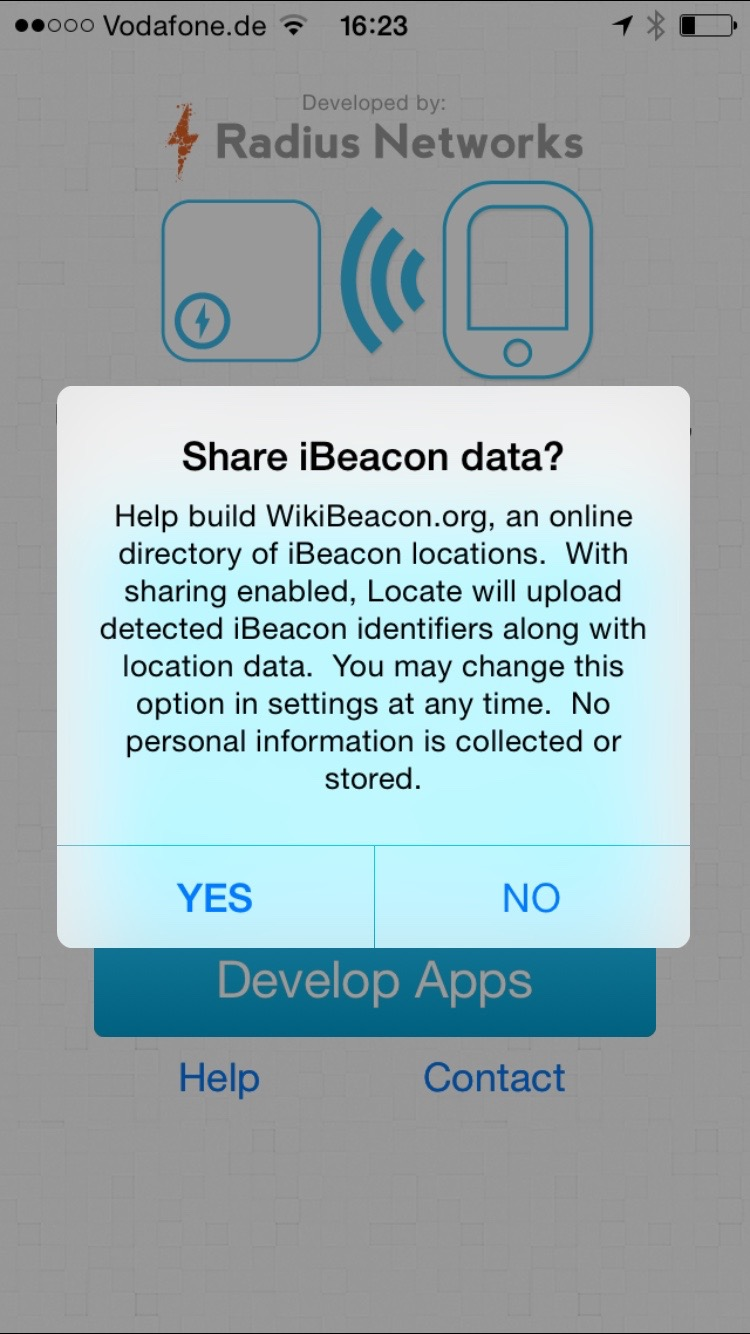
\includegraphics[width=.4\textwidth]{images/experiments/locate.jpg}
	\caption{Radius Networks is collecting Bluetooth beacon location data.}
	\label{fig:locate}
\end{figure}

\subsubsection{Magnetic Flux Sceenshots}



